\documentclass{fp-slides}
% \ifx\pdfoutput\undefined
% % we are running LaTeX, not pdflatex
% \usepackage{graphicx}
% \else
% % we are running pdflatex, so convert .eps files to .pdf
% \usepackage[pdftex]{graphicx}
% \usepackage{epstopdf}
% \fi 
\usepackage{graphics}
\newtheorem{defin}{Definition}
\begin{document}

%%%%%%%%%%%%%%% Define code blocks

% \defverbatim[colored]\factCcode{%
% \begin{lstlisting}[frame=single,language=C]
%   int fact(int n)
%   { int x = 1;
%     while (n > 0)
%      { x = x * n;
%        n = n - 1;
%      }
%     return x;
%   }
% \end{lstlisting}}
% 
% \defverbatim[colored]\factMLcode{%
% \begin{lstlisting}[frame=single]
%   let rec fact n =
%     if n = 0 then 1
%     else n * fact(n - 1);;
% \end{lstlisting}}
% 
% \defverbatim[colored]\badFuncCode{%
% \begin{lstlisting}[frame=single]
%   int rand(void)
%   { static int n = 0;
%     return n = 2147001325 * n + 715136305;
%   }
% \end{lstlisting}}

%%%%%%%%%%%%%%%%%%%%%%

\frame{\titlepage}
\frame{
  \frametitle{Models}
  \begin{defin}
   \textbf{Model} -- a (\textit{simplified}) representation used to explain the workings of a real world system or event
  \end{defin}

\begin{defin}
 A \textbf{mathematical model} is a description of a system using mathematical concepts and language. 
\end{defin}



}

\frame{
\frametitle{Example of models}
\begin{center}
 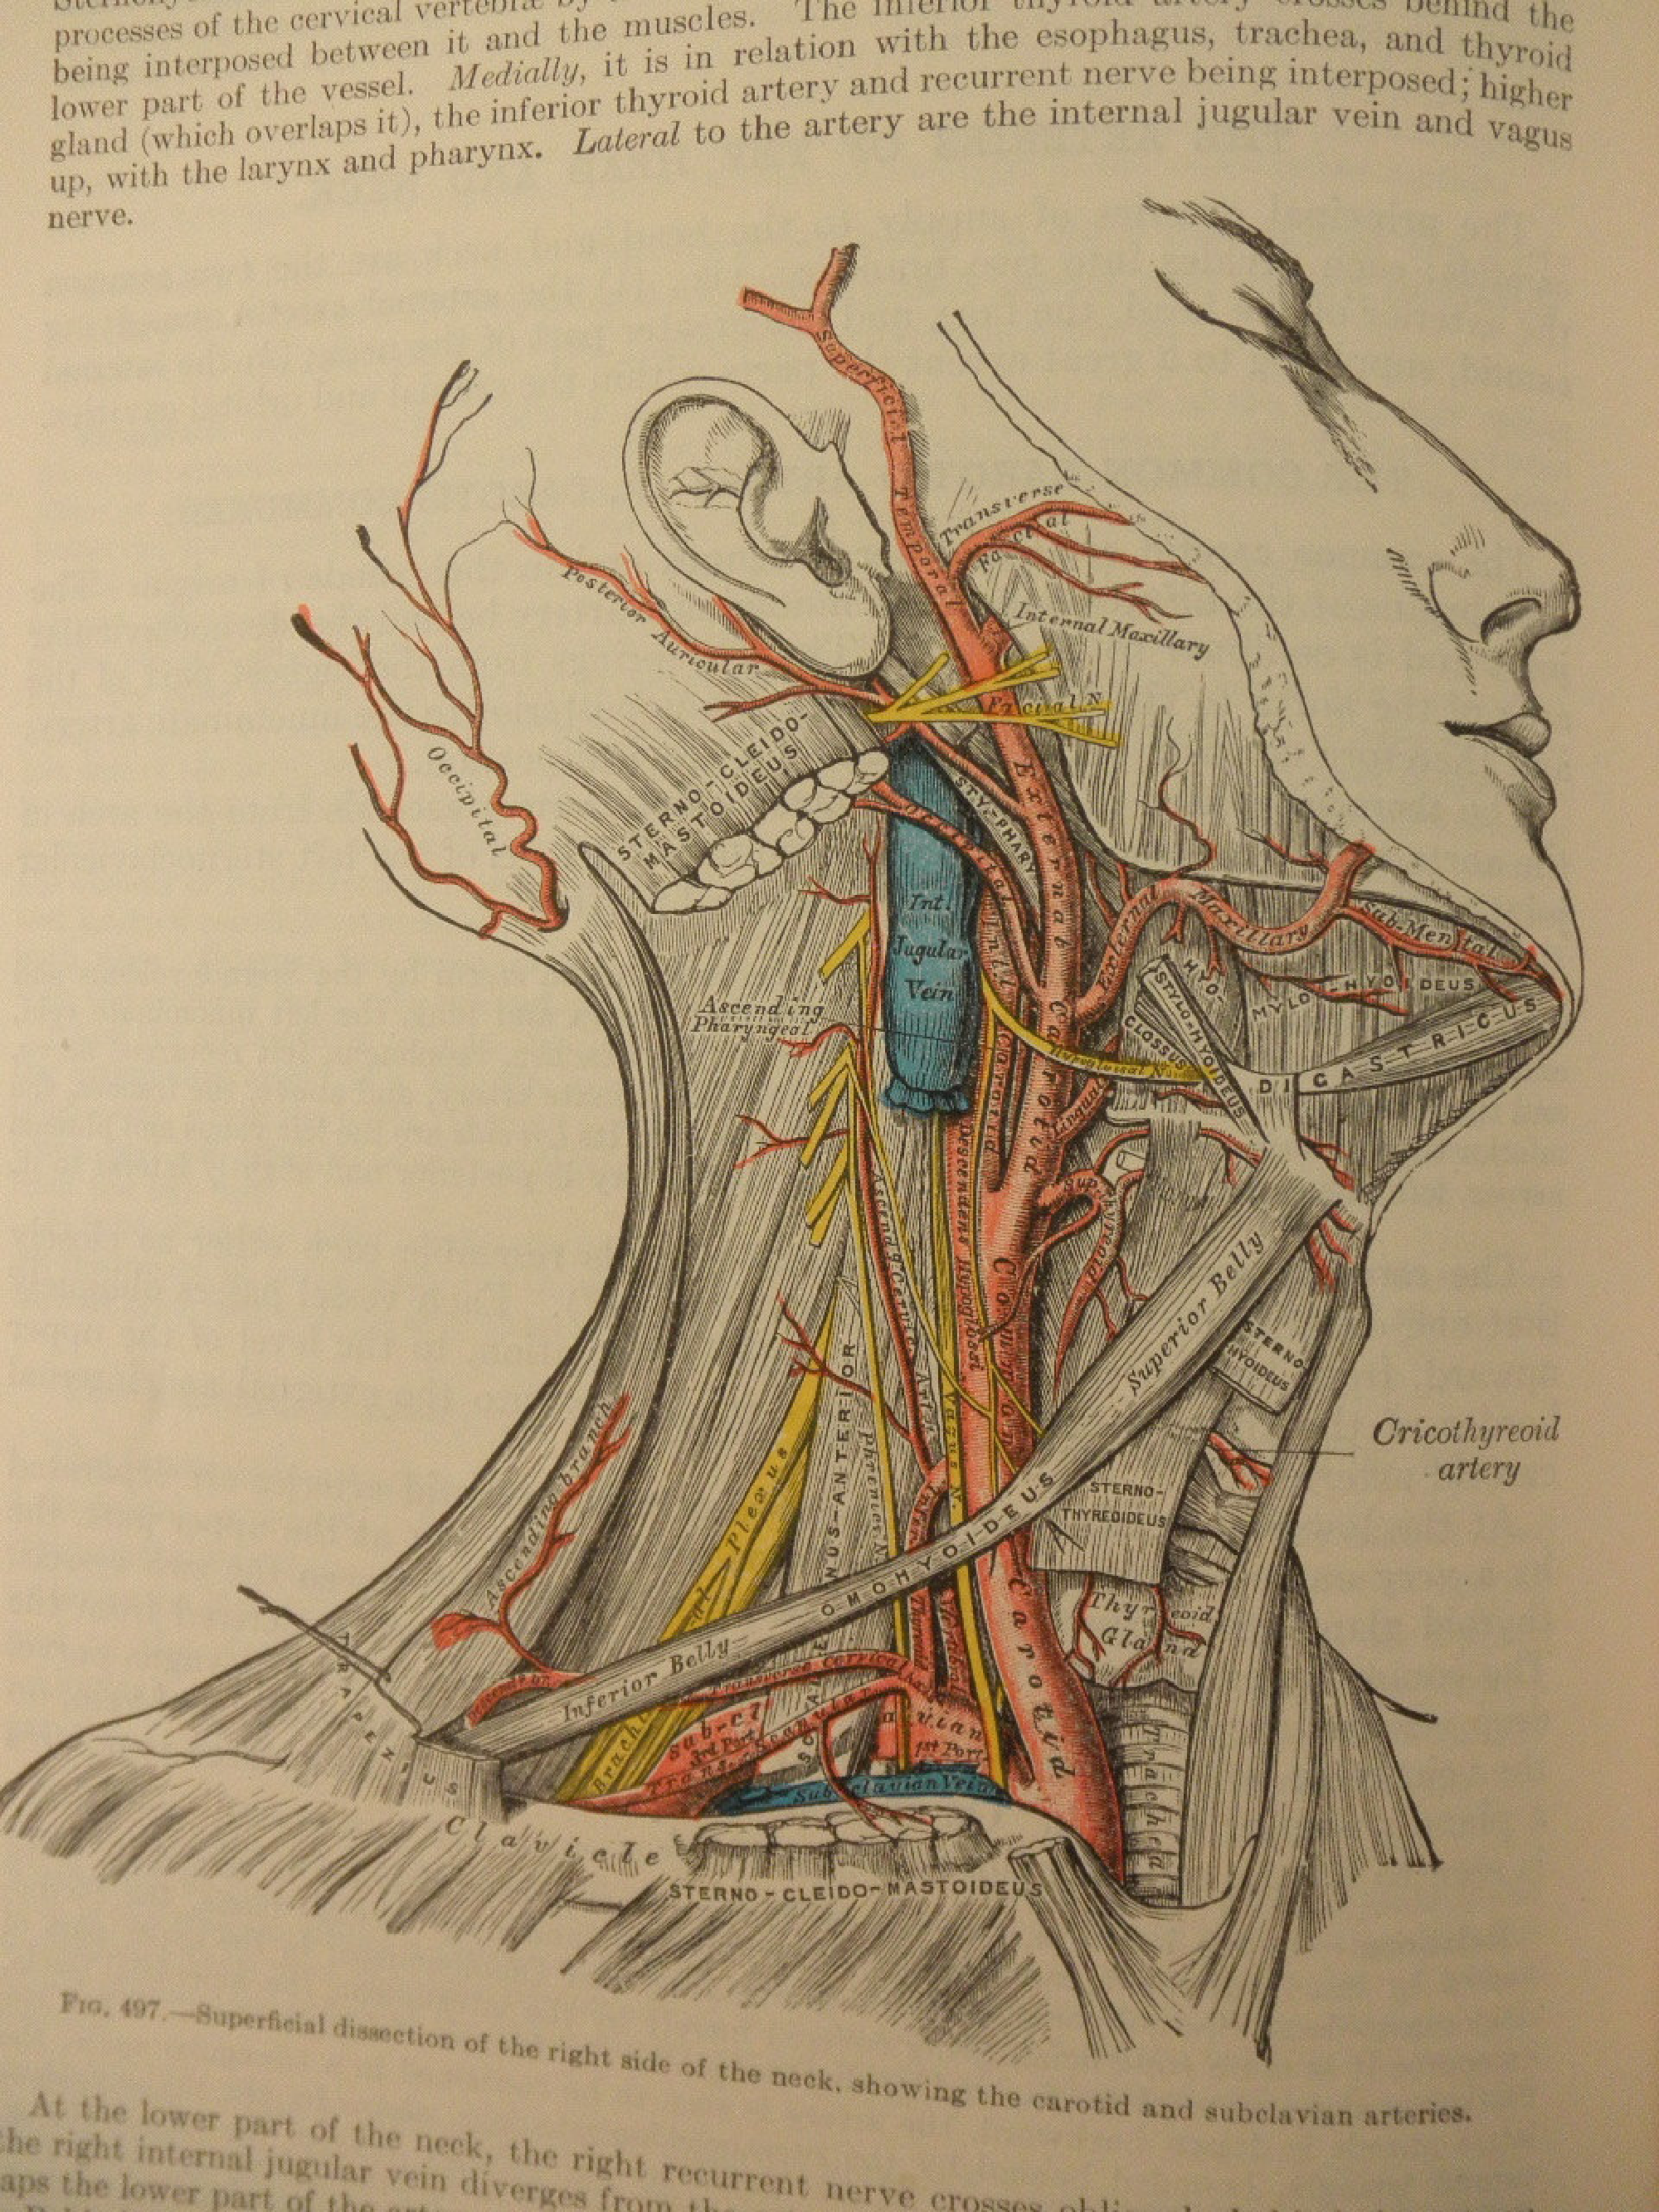
\includegraphics[scale=0.25]{am.pdf}
 % am.pdf: 0x0 pixel, 0dpi, 0.00x0.00 cm, bb=
\end{center}


}


\frame{
\frametitle{Model classifications}
\begin{itemize}
 \item Linear vs. nonlinear
 \item Static vs. dynamic
 \item Explicit vs. implicit
 \item Discrete vs. continuous
 \item \textbf{Deterministic vs. stochastic}
 \item \textbf{Soft vs. hard}
\end{itemize}


}

% \frame{
% \frametitle{Model properties}
% \begin{itemize}
%  \item 
%  \item 
%  \item 
%  
% \end{itemize}
% 
% 
% }


\frame{
\frametitle{Maltus model}
\[
 \frac{dx}{dt} = \alpha x
\]


}

\frame{
\frametitle{Maltus model v2}
\[
 \frac{dx}{dt} = \alpha(1- \frac{x}{k}) x
\]


}
\frame{
\frametitle{Maltusian type models}
\begin{itemize}
 \item \[
 \frac{dm}{dt} = -km
\]
 \item \[
 \frac{dm}{dt} = -km + \frac{dM}{dt}
\]
\[
 \frac{dm}{dt} = -km + rM_0e^{-rt}
\]
$\frac{dM}{dt} = rM$ -- intake from some deposit.

 \item $y(t)$ -- infected. $x(t)$ -- healthy. $x(t) + y(t) = \text{const} = a +b$,  $a= x(0), b = y(0)$
 \[
 \frac{dx}{dt} = - \alpha xy
\]
\[
 \frac{dx}{dt} = - \alpha x (a+b -x)
\]

\end{itemize}



}
\frame{
\frametitle{Predator-prey model}
% \[
%  
% 
% \]
\[
 \left\{\begin{matrix}
\frac{dx}{dt} = \alpha x - \beta xy\\ 
\frac{dy}{dt} = - \gamma y + \delta  x y
\end{matrix}\right.
\]
\begin{itemize}
 \item x is the number of prey (for example, rabbits);
 \item y is the number of some predator (for example, wolfs or foxes);
 \end{itemize}

}

\frame{
\frametitle{Immune system models}

\[
 \left\{\begin{matrix}
\frac{dV_f}{dt}=\nu C_V +nb_{CE}C_VE-\gamma_{VF}FV_f-\gamma_{VM}MV_f-\gamma_{VC}(C^{\ast}-C_V-m)V_f\\ 
\frac{dM_V}{dt}=\gamma_{MV}MV_f-\alpha_MM_V\\ 
\frac{dH_E}{dt}=b^{(E)}_H(\xi(m)\rho_H^{(E)}M_V(t-\tau_H^{(E)})H_E(t-\tau_H^{(E)})-M_VH_E)-b_\rho^{(H_E)}M_VH_EE+\alpha_H^{(E)}(H_E^{\ast}-H_E)\\ 
\frac{dH_B}{dt}=b_H^{(B)}(\xi(m)\rho_H^{(B)}M_V(t-\tau_H^{(B)})H_B(t-\tau_H^{(B)})-M_VH_B)-b_\rho^{(H_B)}M_VH_BB+\alpha_H^{(B)}(H_B^{\ast}-H_B)\\ 
\frac{dE}{dt}=b_\rho^{(E)}(\xi(m)\rho_EM_V(t-\tau_E)H_E(t-\tau_E)E(t-\tau_E)-M_VH_EE)-b_{EC}C_VE+\alpha_E(E^\ast-E)\\ 
\frac{dB}{dt}=b_\rho^{(B)}(\xi(m)\rho_BM_V(t-\tau_B)H_B(t-\tau_B)B(t-\tau_B)-M_VH_BB)+\alpha_B(B^\ast-B)\\ 
\frac{dP}{dt}=b_\rho^{(P)}\xi(m)\rho_PM_V(t-\tau_P)H_B(t-\tau_P)B(t-\tau_P)+\alpha_P(P^\ast-P)\\ 
\frac{dF}{dt}=\rho_FP-\gamma_{FV}V_fF-\alpha_FF\\ 
\frac{dC_V}{dt}=\sigma V_f(C^\ast-C_V-m)-b_{CE}C_VE-b_mC_V\\ 
\frac{dm}{dt}= b_CEC_VE+b_mC_V-\alpha_mm \\
\end{matrix}\right.
\]
}
\frame{
\frametitle{Dixi}

\begin{center}
\Huge Dixi\end{center}
}
\end{document}
